\section{Maps and orientation}
    We will use the maps from the OpenStreetMap (OSM) project\footnote{\url{https://www.openstreetmap.org}}. The maps will be used to determine the surroundings of the robot and whether the current position is suitable for crossing.\\
    OSM is a project that creates and distributes free geographic data. The data is created by the community of users and is available for anyone to use.\cite{OSMwiki}\\
    The map data are expressed by a node, a way, or a relation. A node is a singular point in a map, it could be a landmark, a corner of a building, or a spot on the road. A way is an object created from multiple nodes. It can be either closed or open. Closed ways may represent a park, building, or other types of areas. Open ways commonly represent roads, rivers, or other linear features. The relation is a collection of nodes, ways, or other relations. It is used to describe more complex objects, such as a bus line, a building complex, etc.\\
    We must also clarify the terminology we will use regarding azimuth and heading.\\
    \emph{An azimuth is a bearing, more precisely, a compass bearing from a specific point of observation like a radar station. A heading (in the general case of moving "forward") is the direction your nose is pointed in.}\\
    This description is taken from \cite{heading}. For us, the most important distinction is that while azimuth is obtained from the magnetometer, the heading is calculated from two consecutive GPS coordinates. We also assume that the azimuth is absolute while the heading might be relative. In figure \ref{fig:azi_head}, we can see the difference between the two. The $\varphi_{1}$ is absolute heading, while $\varphi_{2}$ is heading relative to the azimuth $\varphi_{3}$ of the robot. The azimuth and headings are shown for the ENU orientation.
    \begin{figure}[H]
        \centering
        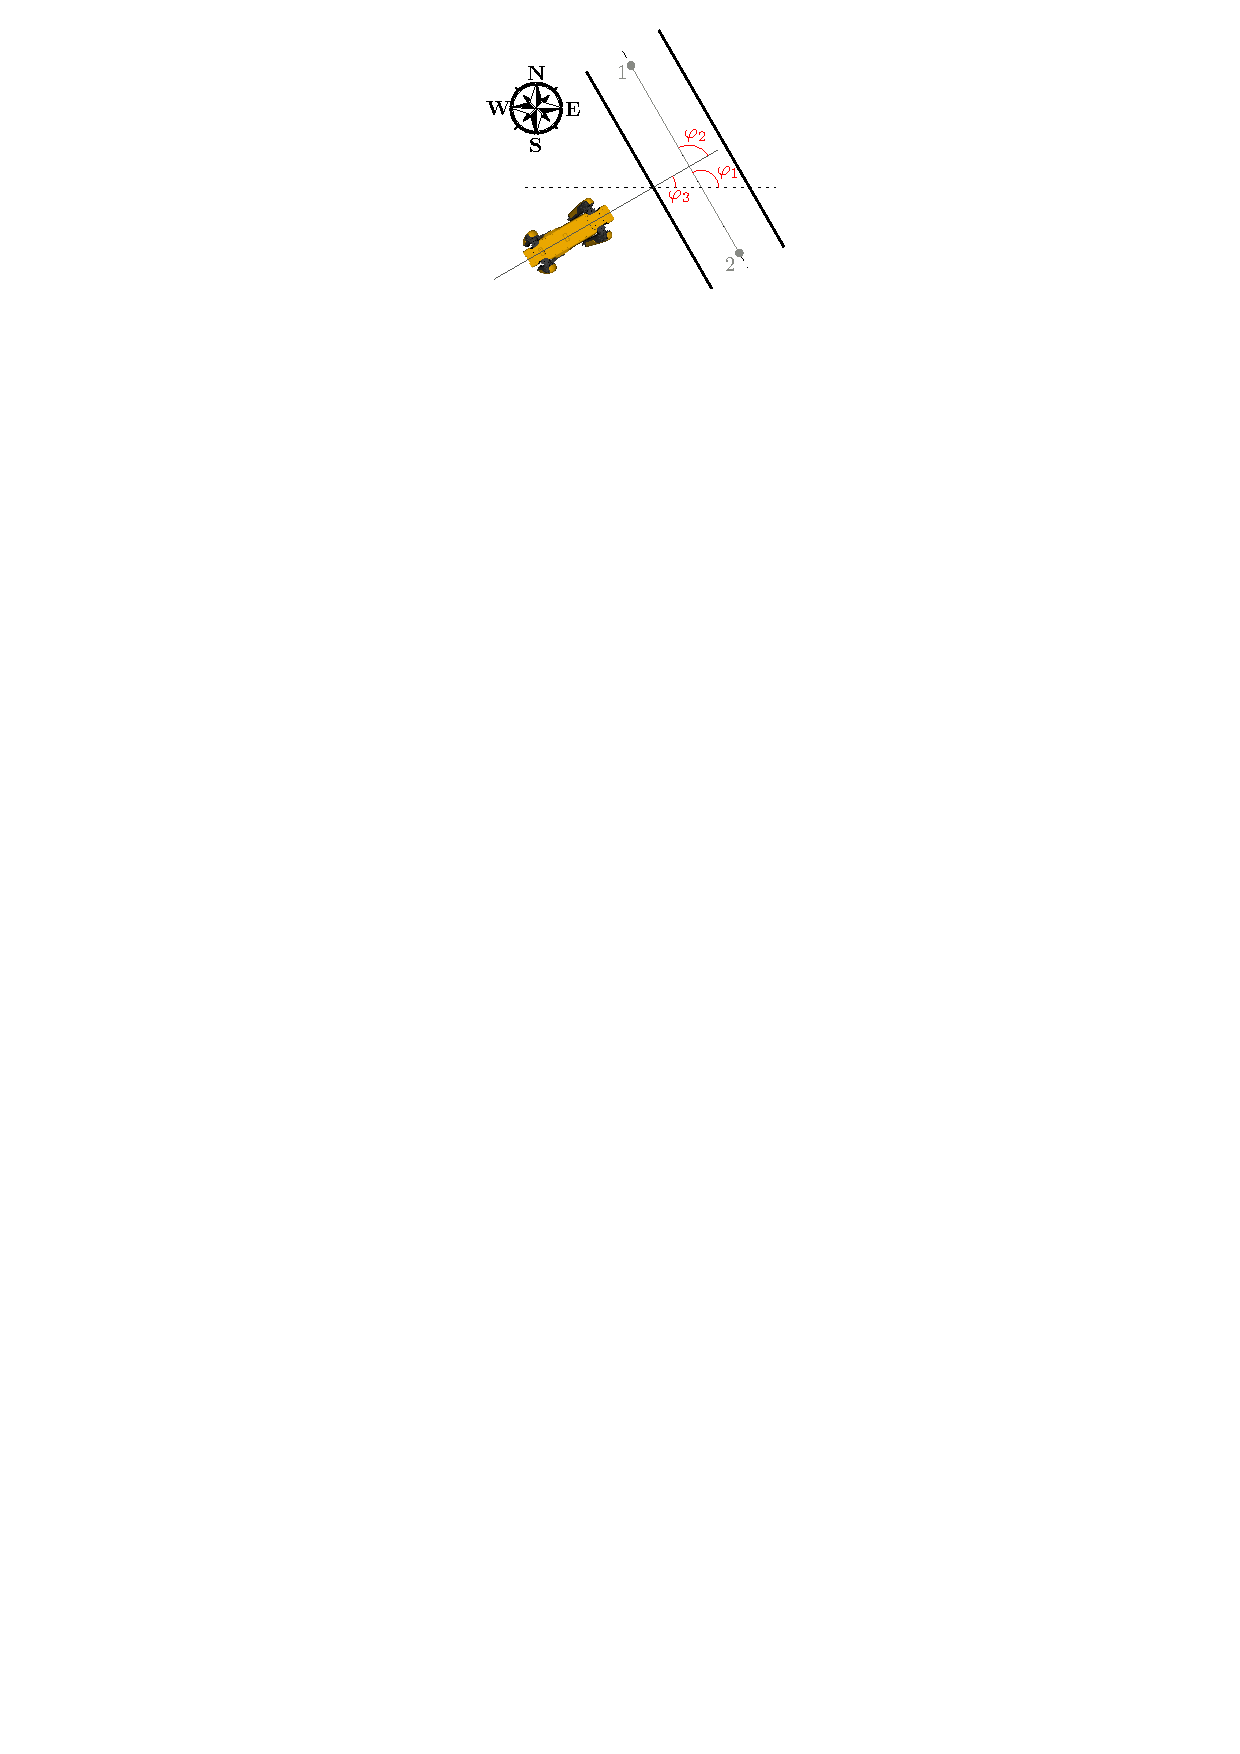
\includegraphics[trim={0 27 0 0}, clip, height=5.9cm]{images/heading.pdf}
        \caption{Difference between azimuth and heading.}
        \label{fig:azi_head}
    \end{figure}
